\section{Appendix}

\subsection{Appendix A - Previous design work}
\label{sec:AppendixA}

  \begin{figure}[H]
    \centering
    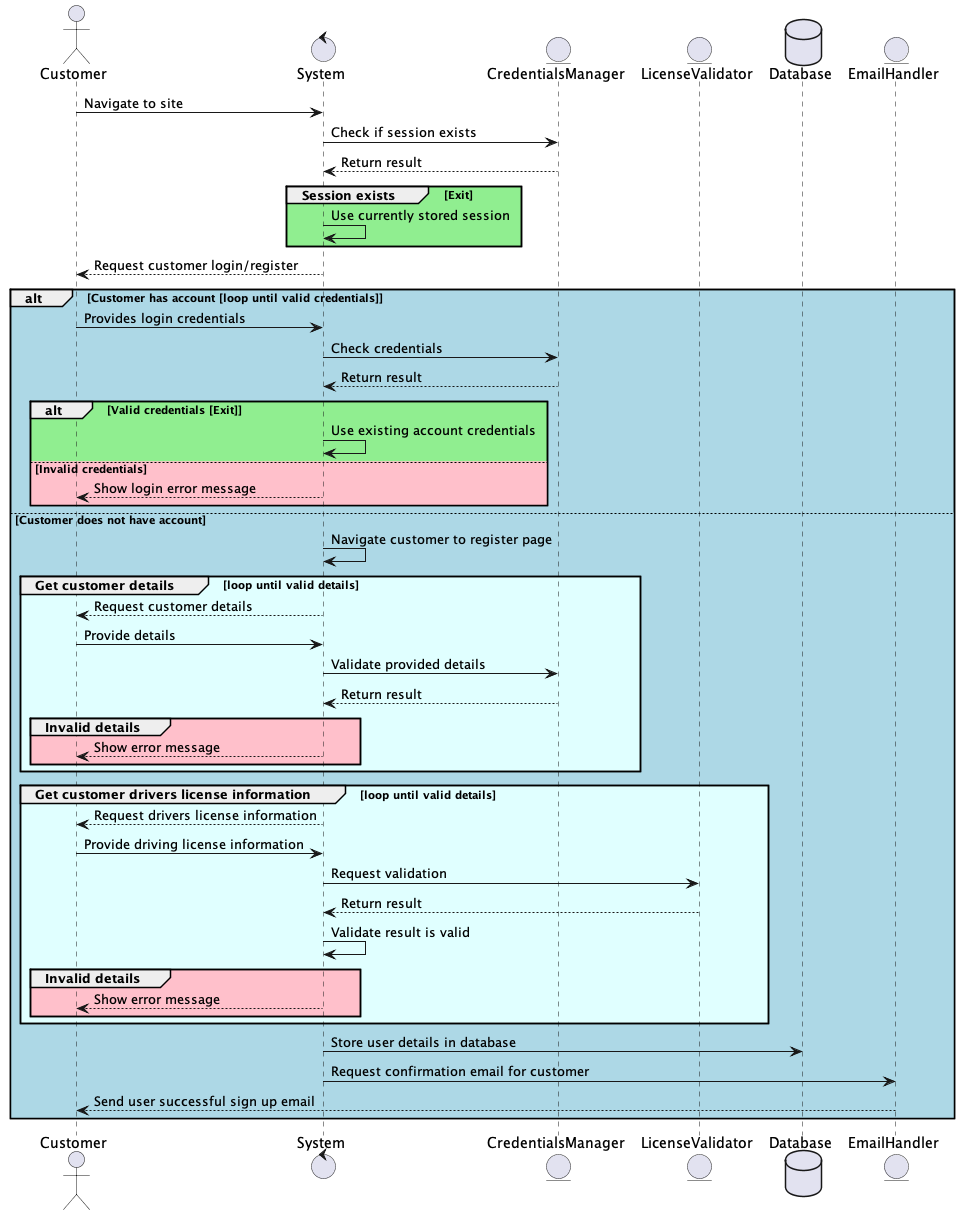
\includegraphics[width=12cm]{assets/Sequence1.png}
    \caption{Sequence diagram for adding a new user, this includes sign in/up.}
    \label{fig:newUserSequence}
  \end{figure}

  \begin{figure}[H]
    \centering
    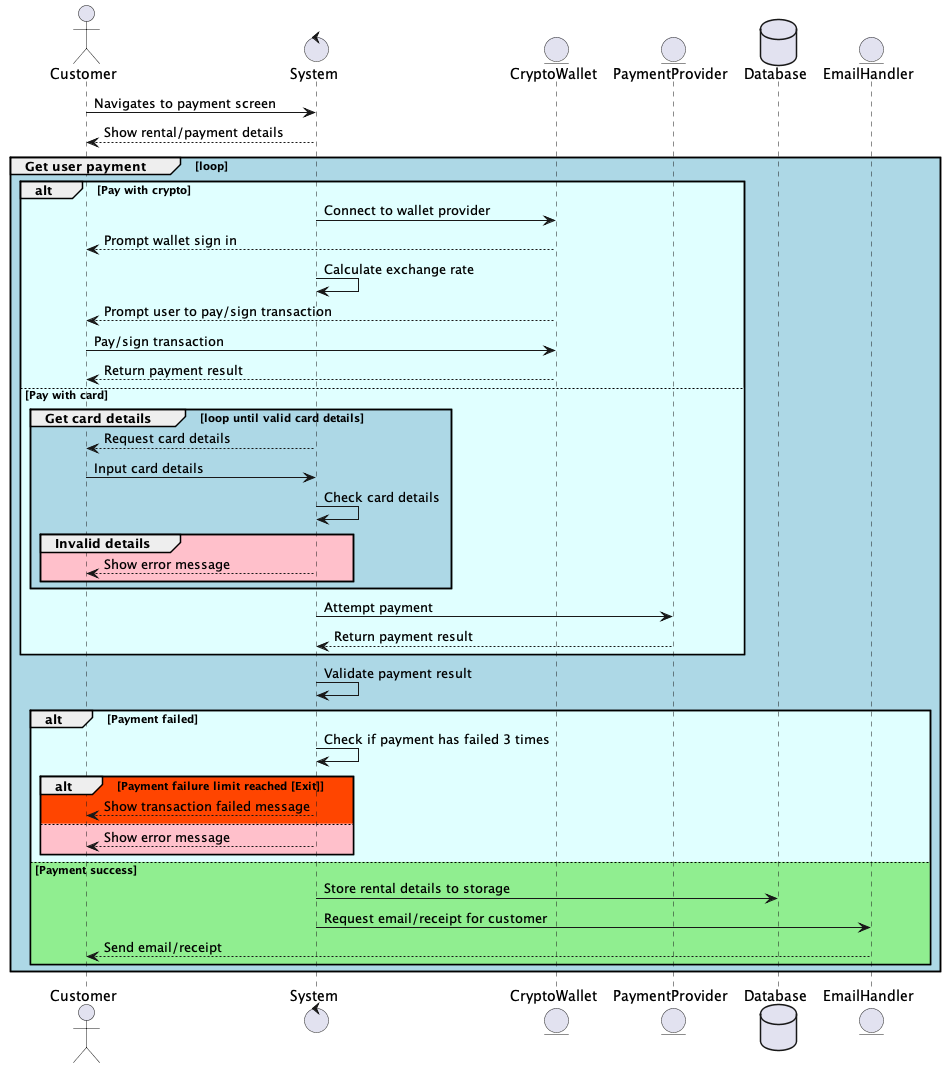
\includegraphics[width=12cm]{assets/Sequence2.png}
    \caption{Sequence diagram for taking a payment.}
    \label{fig:takePaymentSequence}
  \end{figure}

  \begin{figure}[H]
    \centering
    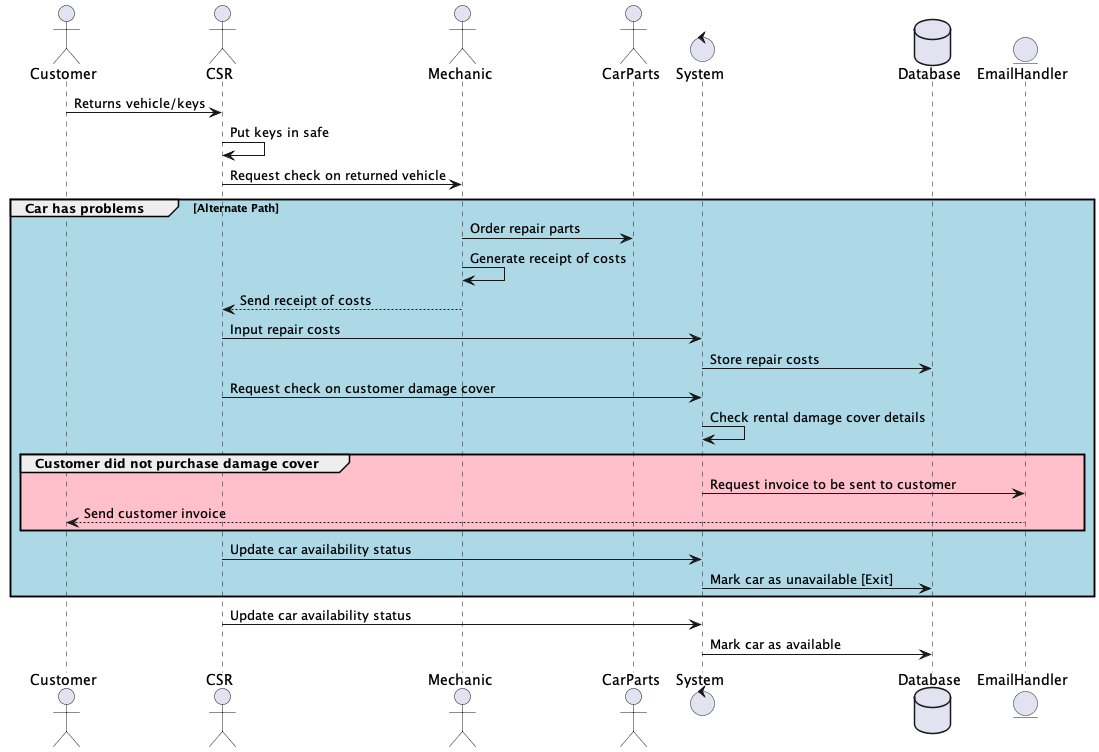
\includegraphics[width=12cm]{assets/Sequence3.png}
    \caption{Sequence diagram for handling the return of a vehicle.}
    \label{fig:vehicleReturnSequence}
  \end{figure}

  \begin{figure}[H]
    \centering
    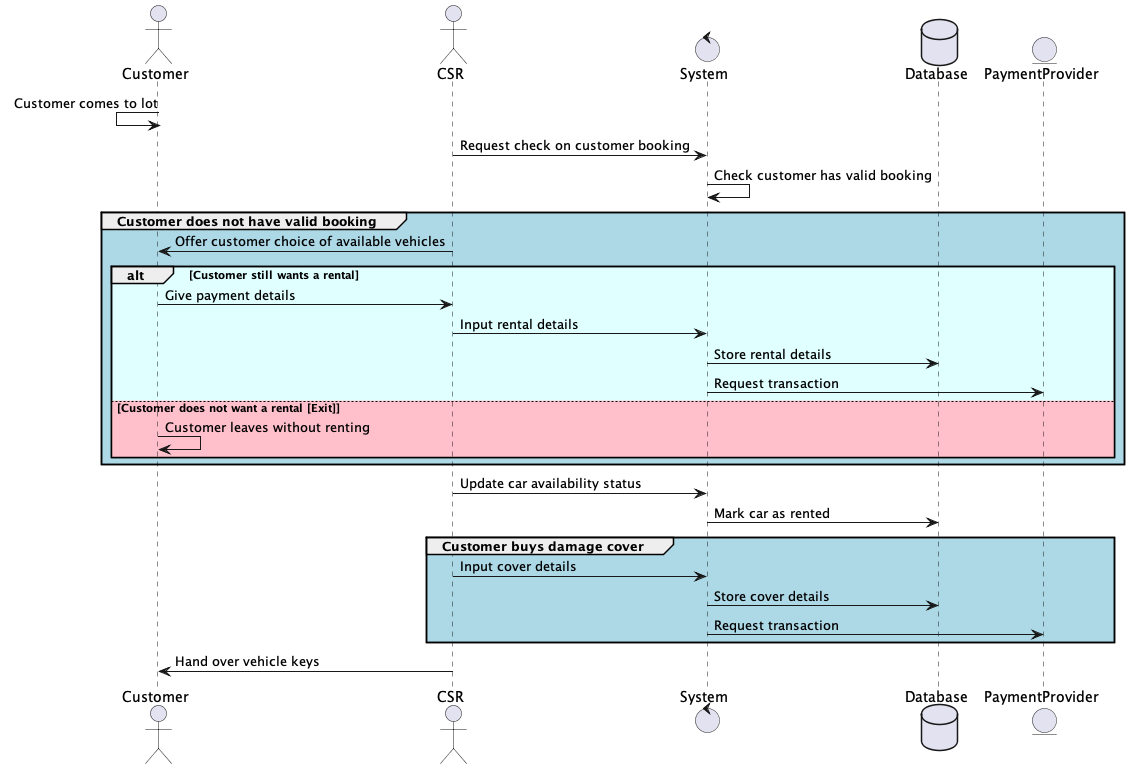
\includegraphics[width=12cm]{assets/Sequence4.png}
    \caption{Sequence diagram for starting a new hire.}
    \label{fig:startHireSequence}
  \end{figure}

  \begin{figure}[H]
    \centering
    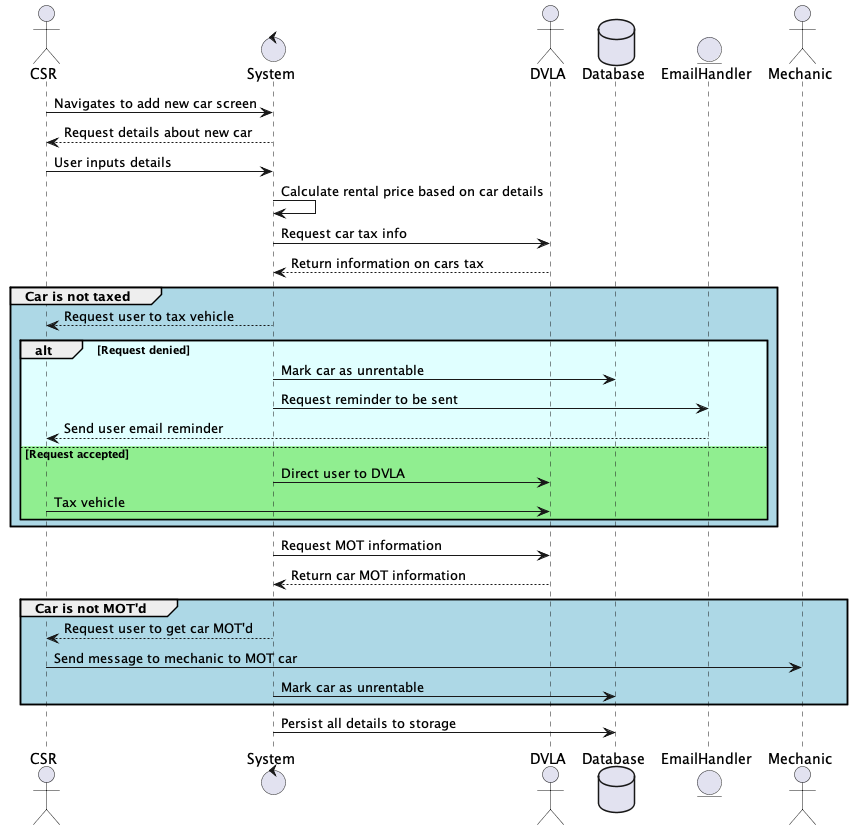
\includegraphics[width=12cm]{assets/Sequence5.png}
    \caption{Sequence diagram for adding a new car to the system.}
    \label{fig:newCarSequence}
  \end{figure}

\subsection{Appendix B - Architectural design of system using AWS}
\label{sec:AppendixB}

  This solution will be built primarily using a cloud-native approach, however as this system is somewhat large there is room for other 
  architectural patterns to be used in sub systems of the overall build. Below is a high level look at how the system could be create using AWS:

  \begin{figure}[H]
    \centering
    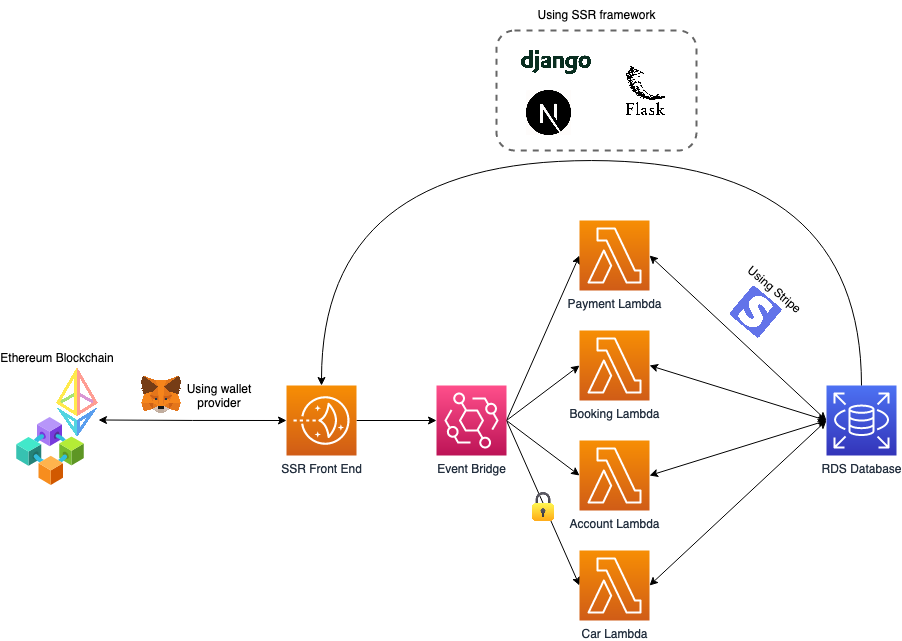
\includegraphics[width=12cm]{assets/architectureEvents.drawio.png}
    \caption{Diagram showing the proposed architecture for the whole system.}
    \label{fig:architecture}
  \end{figure}

  The main component is the Server Side Rendered front end. This can then communicate with the blockchain for crypto transactions using a wallet provider,
  e.g. Metamask [18]. The main functionality is that the front end is then able to send events through EventBridge [19] to individual lambdas [20] for different 
  functionality. These lambdas can then store data into the database. The payment lambda uses Stripe [21] to process payments, and the \textit{'car lambda'} is
  for internal use only, hence the lock on its connection. These topics will be discussed more in the 
  \hyperref[sec:Dependability]{\textbf{Dependability}} section.